\begin{figure}[tbp]
\begin{center}
\includegraphics[width=0.48\textwidth]{figure/powv2d_z1z2_r15r10.eps}
\end{center}
\vspace{-0.7cm}
    \caption{Correlation coefficient r between reconstructed velocity field and real velocity field, 
    assuming a baseline of 100m and serious foregrounds 
    smearing $k_z$ below $~0.08$ h/Mpc and $~0.12$ h/Mpc of redshift 1 and 2 respectively. 
}
\label{fig:v}
\end{figure}

Till now only linear theories are considered in reconstruction, 
however, to extract the lost large scale information, 
we need to consider couplings between different scales in nonlinear theories. 
While there are a great variety of nonlinear effects, 
identifying a single one will help conduct clean reconstruction.   
Here, we present an algorithm to employ 
tidal coupling 
to solve for large scale structures 
\cite{2015:zhu,2012:pen}.  

The evolution of small scale structure is modulated by large scale 
tidal force. 
Consider only the anisotropic influence from tidal force, 
the generated distortions on matter power spectrum will be 
\begin{eqnarray}
\label{eq:powerdistort}
\delta P(\bm{k},\tau)|_{t_{ij}}&=&
\hat{k}^i\hat{k}^jt_{ij}^{(0)}P_{1s}(k,\tau)f(k,\tau)
\end{eqnarray}
where $P_{1s}(k,\tau)$ is the linear powerspectrum; 
$f(k)=2\alpha(\tau)-\beta(\tau)d\ln P/d\ln k$ is the calculated coupling function, 
with $\alpha$ and $\beta$ parameters related to linear growth funcion \cite{2015:zhu}. 
For $z=1$, ($\alpha$,$\beta$)=(0.6,1.3) and ($\alpha$,$\beta$)=(0.4, 0.9) for $z=2$. 
$t_{ij}$ is the tidal force tensor, 
which is symmetric and traceless 
and hence can be decomposed into five components 
%following gravitational lensing procedures.
\begin{eqnarray}
t_{ij}=\left( \begin{array}{ccc}
\gamma_{1}-\gamma_{z} & \gamma_{2} & \gamma_{x}\\
\gamma_{2} & -\gamma_{1}-\gamma_{z} & \gamma_{y}\\
\gamma_{x} & \gamma_{y} & 2\gamma_z
\end{array} \right).
\end{eqnarray}

Therefore, from spatial dependence of the distortions 
$\delta P(\bm{k},\tau)$, 
we could solve for different components of $t_{ij}$. 
And since tidal forces are related to second derivative 
of large scale gravitational potential $\Phi_L$ 
\begin{eqnarray}
\label{eq:tij}
t_{ij}=\Phi_{L,ij}-\nabla^2\Phi_L\delta^D_{ij}/3
\end{eqnarray}
where $_{ij}$ indicates derivative over $x_i$ and $x_j$, 
$\delta^D$ is the Dirac function.

With different components of $t_{ij}$, 
it is straight-forward to reconstruct 
different k modes of the large scale 
density contrast $\kappa_\mathrm{3D}$.
\begin{eqnarray}
    \label{eq:largepoten}
    \kappa_\mr{3D}\sim\nabla^2\Phi_L=\frac{3}{2}\nabla^{-2}\partial_i\partial_j t_{ij}
\end{eqnarray}

Notice that $f(k,\tau)$ increases with $k$ in the interested scales, 
indicating the distortions are more manifest on small scales, 
which explains the feasibility of using existing high $k$ modes in 21cm 
IM fields to extract low $k$ modes. 
\if2=1
We apply identical filters as \ref{15Hongming} 
when selecting the distortions. 
However, \ref{15Hongming} only harness $t_{ij}$ components 
in transverse plane, i.e.$\gamma_1$ and $\gamma_2$ 
as to avoid bias from redshift distortions. 
We use all five components, since there are more intact modes in 
z direction than transverse plane, 
and $\gamma z$ is actually the most important 
shear estimater for the $k_z>k_\perp$ region 
we are most interested in.
\fi
\if1=2
Programming steps:\noindent

(1) Gaussianize the field, taking 
$\delta_g=\mathrm{ln}(1+\delta)$. 
This is to allieviate the problem that filter $W_i$ in Eq.(\ref{eq:wi}) heavily weights high density regions.

(2) Following gravitational lensing procedures, decompose the symmetric, traceless tidal force tensor into 5 components, 

(3) Select density distortions caused by tidal force, 
by convolving $\delta_g$ with a filter $W_i$ 
deduced from Eq.(\ref{eq:powerdistort}) 
\begin{eqnarray}
\delta^{w_i}_g(\bm{k})=W_i(\bm{k})\delta_g(\bm{k}) 
\end{eqnarray}
\begin{eqnarray}
\label{eq:wi}
W_i(\bm{k})=i \bigg[\frac{P(k)f(k)}{P_{tot}^2(k)}\bigg]^{\frac{1}{2}}\frac{k_i}{k}
=S(k)\frac{k_i}{k}\nonumber
\end{eqnarray}
$P_{tot}=P+P_{noise}$ is the observed matter powerspectrum, 
and P is theoretical matter powerspectrum,
%\footnote{The value of $S(k)$ on different scales could be seen in Appendix 1.}

(4) Estimate the 5 tidal tensor components from quadratic statistics.
\begin{eqnarray}
\label{eq:gamma}
\hat{\gamma}_1(\bm{x})&=&
[{\delta}^{w_1}_g(\bm{x}){\delta}^{w_1}_g(\bm{x})-
{\delta}^{w_2}_g(\bm{x}){\delta}^{w_2}_g(\bm{x})],\nonumber\\
\hat{\gamma}_2(\bm{x})&=&
[2{\delta}^{w_1}_g(\bm{x}){\delta}^{w_2}_g(\bm{x})],\nonumber\\
\hat{\gamma}_x(\bm{x})&=&
[2{\delta}^{w_1}_g(\bm{x}){\delta}^{w_3}_g(\bm{x})],\\
\hat{\gamma}_y(\bm{x})&=&
[2{\delta}^{w_2}_g(\bm{x}){\delta}^{w_3}_g(\bm{x})],\nonumber\\
\hat{\gamma}_z(\bm{x})&=&
\frac{1}{3}[(2{\delta}^{w_3}_g(\bm{x}){\delta}^{w_3}_g(\bm{x})\nonumber\\
&&-{\delta}^{w_1}_g(\bm{x}){\delta}^{w_1}_g(\bm{x})
-{\delta}^{w_2}_g(\bm{x}){\delta}^{w_2}_g(\bm{x}))],\nonumber
\end{eqnarray}

(5) Reconstruct large scale density contrast $\kappa_\mr{3D}$ from tidal tensor:
\begin{eqnarray}
\kappa_\mr{3D}(\bm{k})=\frac{1}{k^2}
&&[(k_1^2-k_2^2)\gamma_1(\bm{k})+2k_1k_2\gamma_2(\bm{k})\nonumber\\
&&+2k_1k_3\gamma_x(\bm{k})+2k_2k_3\gamma_y(\bm{k})\\\nonumber
&&+(2k_3^2-k_1^2-k_1^2)\gamma_z(\bm{k})].
\end{eqnarray}

(6) Correct bias and suppress noise with a Wiener filter.

Due to the foregrounds, the noise in $z$ direction will be different from $x$,$y$ direction, therefore we apply an anisotropic Wiener filter.
\begin{eqnarray}
	\label{eq:wiener}
    \hat \kappa_{c}(\bm{k})=\frac{\kappa_{\mathrm{3D}}(\bm{k})}{b(k_\perp,k_\parallel)}W(k_\perp,k_\parallel)\ ,
\end{eqnarray}
Bias $b(k_\perp,k_\parallel)=P_{\mathrm{k3D,}\delta}/P_\delta$ 
is the cross powerspectra between reconstructed field $\kappa\mathrm{3D}$ and original field $\delta$, 
Wiener filter $W(k_\perp,k_\parallel)=P_\delta/(P_{\mathrm{k3D}}/b^2)$.

Here $\hat \kappa_{c}$ is the output large scale density contrast we obtain from tidal reconstruction.
We use it to calculate velocity $\hat v_z^{\mathrm{tide}}$.
\fi
